\documentclass{article}

\usepackage{listings}
\usepackage{color}
\usepackage{graphicx}
\usepackage{float}
\usepackage{amsmath}
\usepackage{subfig}
\usepackage{cite}
\usepackage{url}

\begin{document}

\title{Image Analysis - TP2 - Local Filtering and Histograms}

\author{Jander Nascimento, 
\and Raquel Oliveira}

\maketitle

\section{Filtering}
	
	\subsection{Binomial}

		Binomial filter uses pascal's triangle to create a filter. This filter has the blurry effect with some differences.
One example of a 3x3 Binomial filter can be seen in the Figure \ref{3x3binomial}.

\begin{figure}[H]
  \begin{center}
  \begin{tabular}{ | c | c | c | }
    \hline
    1 & 2 & 1 \\ \hline

    2 & 4 & 2 \\ \hline

    1 & 2 & 1 \\
    \hline
  \end{tabular}
  \end{center}
  \caption{3 x 3 Binomial filter\label{3x3binomial}}\end{figure}

		To apply this kernel to the image, it is necessary to perform the convolution in the original image with this kernel.

		This kernel is used to remove the noise in image, but it do not preserves the edges of the image. 
		
	\subsection{Median}

		With a purpose of noise reduction, in certain situations it can preserve the edges while reduce the noise of the image.

		For this reason this kind of filter is regularly used as a pre-traitement for edge detection.

		The Median filtering differ from others filters in the way it is applied to the image. While other filters are defined by kernels, the Median filter depends on each sector of the image analized to generate a new kernel.

		Median kernel is copy a certain sector of the image analized and change the value of the central pixel in the original image. 

		The central pixel in the original image receives the median value of the kernel. It is possible to do it by simply sorting the content of the kernel and assign the value in the middle (central position of the kernel) to the original image. 

	\subsection{Median versus Binomial}

		\begin{figure}[H]
		  \centering
		  \subfloat[Binomial]{\label{fig:binomial}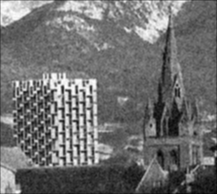
\includegraphics[width=0.4\textwidth]{../image/church_binomial}}                
		  \subfloat[Median]{\label{fig:median}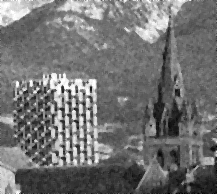
\includegraphics[width=0.4\textwidth]{../image/church_median}}
		  \caption{Removing noise}
		  \label{fig:removingnoise}
		\end{figure}		

	In the Figure \ref{fig:removingnoise} we applied Binomial and Median filter separetely. 
	Median preserves the edges better than the Binomial, although the Binomial preserves some central details in the image. 
	This behaviour can be seen in the window at the chappel, in the Binomial is possible to see the borders of the line, while in the Median this detail is not displayed. 

\section{Histogram}

	The histogram is an important tool when dealing with image analysis. It shows the color distribution of a certain image regarding to its color spectrum. The 		histogram is represented in a Cartesian, where x axis is the color spectrum and y represents the number of pixels that have such intensity.

	In this pratical work, we wrote a function in c that computes the intensity histogram. The function has the following steps:
	\begin{itemize}
  		\item take from the main argument the name of the file that will be analised.
  		\item create a matrix (with the dimensions of the image) to store the pixels' intensity of the image
  		\item go through such matrix and count the number of pixels in each intensity at the spectrum of the color (from 0 to 255)
  		\item store that in an array of 256 positions.
  		\item display such array on the standard output device (screen)
	\end{itemize}

	\subsection{Stretching}

	The histogram stretching is a technique by which the color histogram is used to evaluate and possibly change the color intensity range. This enhances the 		detail level of some images that might appear too dark or too bright. This is done by spreading the pixels to use the entire color spectrum.
	
	To apply the stretching, the only variables we must know is the minimum and maximum color in the current histogram, and minimum and maximum color in the 		enhanced histogram, or we may translate as a new position for the minimum and maximum colors. 

	In this pratical work, we wrote a function in c that transforms an image with the histogram stretching. The function has the following steps:
	\begin{itemize}
  		\item take from the main argument the name of the file that will be analised.
  		\item create a matrix (with the dimensions of the image) to store the pixels' intenxity of the image
  		\item in the matrix, find the current range minimum of the image({\it $current_{min}$}), which is the mininum intensity of the spectrum of the color 			that is used in the image
  		\item find also the current range maximum of the image({\it $current_{max}$}), which is the maximum intensity of the spectrum of the color that is 			used in the image
  		\item for each pixel of the image, calculate its new intensity based on the stretching's formula:
		\begin{equation}
			y[n]=new_{min}+\frac{new_{max}-new_{min}}{current_{max}-current_{min}}*(x[n]-current_{min})
			\label{eq:stretching}
		\end{equation}
	
		where: 
			\begin{itemize}
	  			\item {\it n} is the pixel		
	  			\item {\it $new_{min}$} is 0;
	  			\item {\it $new_{max}$} is 255; 
	  			\item {\it x[n]} is the current intensity of the pixel.
			\end{itemize}
	\end{itemize}

	\begin{figure}[H]
	\centering
	\subfloat[Original Image]{\label{fig:original}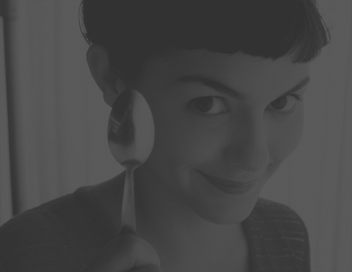
\includegraphics[width=0.4\textwidth]{../image/amelie}}                
	\subfloat[Stretched Image]{\label{fig:stretched}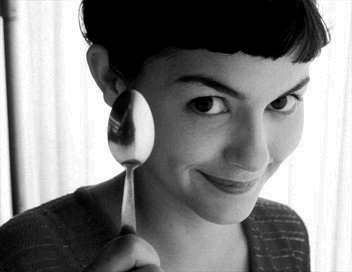
\includegraphics[width=0.4\textwidth]{../image/amelie_stretched}}
	\caption{Stretching Transformation}
	\label{fig:stretching}
	\end{figure}

	\subsection{Equalization}

	Histogram equalization is a method in image processing of contrast adjustment using the image's histogram. This method usually increases the global contrast 		of many images, especially when the usable data of the image is represented by close contrast values. Through this adjustment, the intensities can be better 		distributed on the histogram. This allows for areas of lower local contrast to gain a higher contrast. Histogram equalization accomplishes this by 		effectively spreading out the most frequent intensity values.

	In this pratical work, we wrote a function in c that transforms an image with the histogram equalization. The function has the following steps:
	\begin{itemize}
  		\item compute the histogram of the image (following the steps of the question before)
  		\item create an array to store the cumulative distribution function of the histogram, which is the values of the histogram in a cumulative way.
  		\item in such array, find the minimun value at all the spectrum of the color (cdfmin)
  		\item for each pixel of the image, calculate its new intensity based on the equalization formula:
			\begin{equation}
				h[v]= round \left( \frac{cdf(v)-cdf_{min}}{(M * N) - cdf_{min}} * (L-1) \right) 
			\label{eq:equalization}
			\end{equation}
			
			where:		
			\begin{itemize}
	  			\item {\it v} is the current intensity of the pixel		
		  		\item {\it cdf(v)} is the value of such intensity in the array that stores the acumulated values of the histogram
		  		\item {\it M} is one dimension of the image		
		  		\item {\it N} is the other dimension of the image
		  		\item {\it L} is the number of color levels used (in most cases, 256)
			\end{itemize}
	\end{itemize}

	\begin{figure}[H]
	\centering
	\subfloat[Original Image]{\label{fig:original}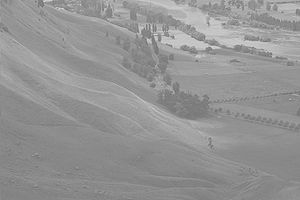
\includegraphics[width=0.4\textwidth]{../image/view_unequalized}}                
	\subfloat[Stretched Image]{\label{fig:stretched}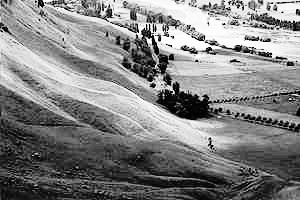
\includegraphics[width=0.4\textwidth]{../image/view_equalized}}
	\caption{Equalization Transformation}
	\label{fig:stretching}
	\end{figure}

\end{document}

